\documentclass{beamer}
\newcommand{\RR}{\mathbb{R}}
\title{RL Chapter 3 - Finite Markov Decision Process}
\author{Finn Ye}
\date{Feb 2025}

\begin{document}

\frame{\titlepage}

\begin{frame}{Introduction}
\begin{enumerate}
    \item Actions influence not only immediate rewards, but also subsequent situations.
    \item Trade off between immediate and delayed reward.
\end{enumerate}
\end{frame}

\begin{frame}{Definition}
\begin{enumerate}
    \item The \textbf{agent} is the learner and decision maker.
    \item The \textbf{environment} is everything the agent interacts with. The environment usually include anything that cannot be arbitrarily changed by the agent.
\end{enumerate}
\end{frame}

\begin{frame}{Setup}
    \begin{enumerate}
        \item Time steps are discrete: $t=0,1,2,\cdots$
        \item At each step, the agent receives information on the current state $S_t\in S$ and selects their action $A_t \in A(S_t)$.
        \item Depending on the action, the agent receives a reward $R_{t+1}\in R\subset\RR$ and moves to the next state $S_{t+1}$.
        \item The \textbf{dynamics} can be described using the probability $p$ defined by
        \[
        p(s',r|s,a)=P\{S_t = s', R_t = r|S_{t-1}=s,A_{t-1}=a\}
        \]
    \end{enumerate}

    A sequence follows like $S_0,A_0,R_1,S_1,A_1,R_2,S_2,\cdots$
    
    \begin{minipage}{\linewidth}
    \centering
    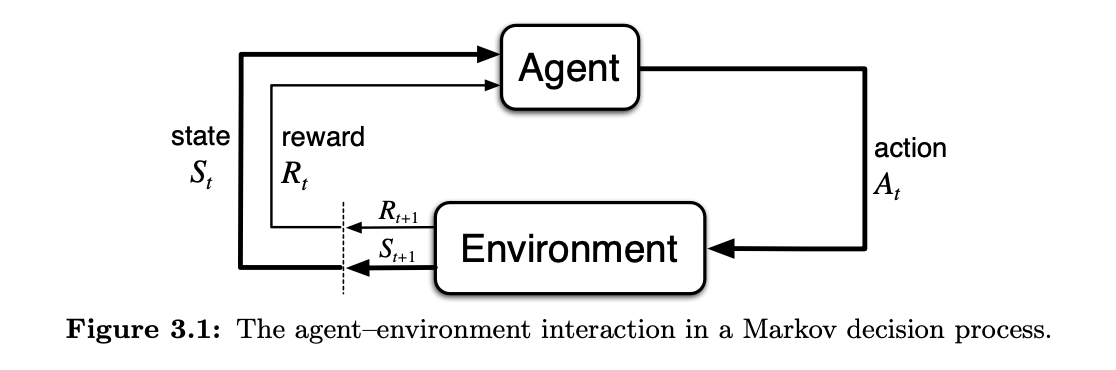
\includegraphics[width=0.8\linewidth]{F31.png}
    \end{minipage}
\end{frame}

\begin{frame}{Returns}
    \begin{enumerate}
        \item \textbf{Episodes} are cases where there is a natural notion of final time step.
        \item \textbf{Continuing Tasks} are those going on continuously without limit.
        \item The agent's goal is to maximize the expected discount return:
        \[
        G_t \equiv R_{t+1} + R_{t+2} + \cdots = \sum_{k=0}^\infty \delta^k R_{t+k+1}
        \]
        where $\delta\in[0,1]$ is the discount rate. (I refuse to use $\gamma$ to represent it.)

        \item By introducing absorbing state after the terminal nodes for episodes, we can use the same notation to describe both situations.
    \end{enumerate}
\end{frame}

\begin{frame}{Policies and Value Functions}
\begin{enumerate}
    \item A \textbf{policy} is a mapping from states to probabilities of selecting each possible actions. $\pi(a|s)$ describes the probability that $A_t = a$ given $S_t=s$ when the agent follows policy $\pi$.
    \item The \textbf{value function} of a state $s$ under policy $\pi$ is denoted $v_\pi(s)$.
    \item The value function $v_\pi$ is the unique solution to its Bellman equation defined by 
    \[
    v_\pi(s) = \sum_a \pi(a|s) \sum_{s',r}p(s',r|s,a)[r+\delta v_\pi(s')],\quad \forall s\in S
    \]
\end{enumerate}
\end{frame}

\begin{frame}{Grid World (Example 3.5)}
The world is defined as a $5\times 5$ grid. At each cell on the grid, the actions are $\{\text{north, south, east, west}\}$.\\

If the agent takes an action that will bring them off grid, their location will remain unchanged and receive a reward of $-1$.

Any action at state $A$ brings the agent to $A'$ and gives a reward of 10. Any action at state $B$ brings the agent to $B'$ and gives a reward of $5$. All other actions give a reward of 0.
\end{frame}

\begin{frame}{Pseudo Code for Grid World}
    \begin{itemize}
        \item $\pi:$ each direction is played with same probability.
        \item Define the world size, possible actions, and rewards.
    \end{itemize}
    \begin{enumerate}
        \item Solve $v_\pi$ with linear system
            \begin{itemize}
                \item Solve for 
                \[
                v_\pi(s) = \sum_a \pi(a|s) \sum_{s',r}p(s',r|s,a)[r+\delta v_\pi(s')],\quad \forall s\in S
                \]
            \end{itemize}

        \item Solve $v_\pi$ by value function iteration
            \begin{itemize}
                \item Set an initial guess for $v_k$.
                \item \textbf{Loop} 
                
                Update $v_k$ with Bellman equation using $\pi$ given.

                If $|v_{k+1}-v_k|$ is small enough, the loop ends and we find the solution.
            \end{itemize}
    \end{enumerate}
\end{frame}

\begin{frame}{Pseudo Code for Grid World}
    \begin{itemize}
        \item We want to find the optimal policy $\pi^*$ and corresponding $v_\pi^*$.
        \item Set an initial guess for $v_k$.
        \item \textbf{Loop}

        Sweeping through all $a\in A$ to find the maximum value possible and update $v_{k+1}$ with it.

        If $|v_{k+1}-v_k|$ is small enough, the loop ends and we find the optional $v_\pi^*$.

        \item Giving the optimal value function, sweep through possible actions to find the action that yields the optimal value. This gives the optimal policy $\pi^*$. 
    \end{itemize}
\end{frame}
\end{document}